% Enumerate a fleshed-out view of my work history, including:
% 1) What the company is/was
% 2) What I did there
% 3) What I took away from the experience
% 4) Artifacts supporting the descriptions
\subsection{\textbf{CTO} at \shstandout{Pavia Systems, Inc.} \shyears{[2015-PRESENT]}}
Pavia Systems\footnote{\href{http://www.paviasystems.com/}{The Pavia Site}} specializes in creating technology systems for organizations in the transportation infrastructure industry.  Pavia's customers include large Departments of Transportation, Contractors, Equipment Manufacturers, and Materials companies all with ties to the industry.  Pavia is highly specialized with core expertise in technology, industry issues, and education, making it uniquely qualified to deliver best-in-breed technology systems.  Pavia has \pstandout{provided opportunities to implement products and data research tools in large-scale government projects}.

\subsection{\textbf{Board Member \& Cofounder} at \shstandout{DocuCluster, Inc.} \shyears{[2011-PRESENT]}}
DocuCluster\footnote{\href{http://www.docucluster.com/}{The DocuCluster Site:}\\http://bit.ly/1cCOAVO} is a vertical market software company in the oil \& gas exploration industry.  Originally this was an informal collaboration with my cofounder to research automatically generating graphs of complex textual documents via OCR.  This has blossomed into a great ``when we want to'' weekend job for stretching the brain in a very complex problem space.  Entirely self-funded, we aren't in a hurry to grow a huge organization, instead focusing on designing and building quality products.  My work at DocuCluster has \pstandout{been a revelation in understanding systems for presenting large bodies of complex search results to users in a meaningful way}.
\begin{marginfigure}%
  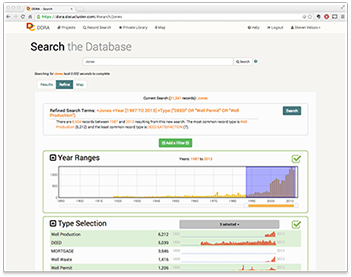
\includegraphics[width=\linewidth]{DORARefine}
  \caption{The DORA Search Product}
  \label{fig:DoraProduct}
\end{marginfigure}

Using modern technologies such as Lucene, Solr, neo4j, node.js and mapnik we provide real-time access to complex reports uniting huge bodies of data.  The standard industry process for assembling these reports requires multiple departments and weeks of lead time.

\subsection{\textbf{Chief Architect} at \shstandout{Promethean, Inc.} \shyears{[2010-2014]}}
Promethean\sidenote{\href{http://www.prometheanworld.com/}{Promethean, Inc. Site}\\ http://bit.ly/Ls8dug} is a global education technology company, primarily in the interactive whiteboard business.  When Promethean acquired SynapticMash, I shifted into the Chief Architect position at Promethean.  My first task was to retool the SynapticMash education software platform to be a part of the Promethean product ethos; this product became ActivProgress.  Over the course of four years my responsibilities grew, ultimately running teams in three global locations delivering five distinct software product lines.  These products included:
\begin{itemize}
\itemsep-0.5em
\item{Highly scalable web software\sidenote{\href{http://www.ednetinsight.com/news-alerts/world-headlines/promethean-agreement-with-mexican-government.html}{ActivProgress Mexico}\\ http://bit.ly/19AP2sx}}
\item{Strategic software partnerships deliverables\sidenote{\href{http://www.examiner.com/article/mcgraw-hill-s-power-of-u-potential-meets-possibility}{McGraw-Hill Power of U}\\ http://exm.nr/1eRSwqw}}
\item{Local network server software}
\item{Mobile applications for iOS, Android and Win8 RT\sidenote{\href{http://www.prometheanworld.com/us/english/education/products/assessment-and-student-response/activengage2/}{ActivEngage 2}\\ http://bit.ly/1axvUtL}}
\item{An internet-based license management server}
\item{Hardware drivers for Windows, Linux and Mac OS/X}
\item{Thick productivity software we bundle with our hardware}
\end{itemize}

\begin{centering}
\begin{figure}%
  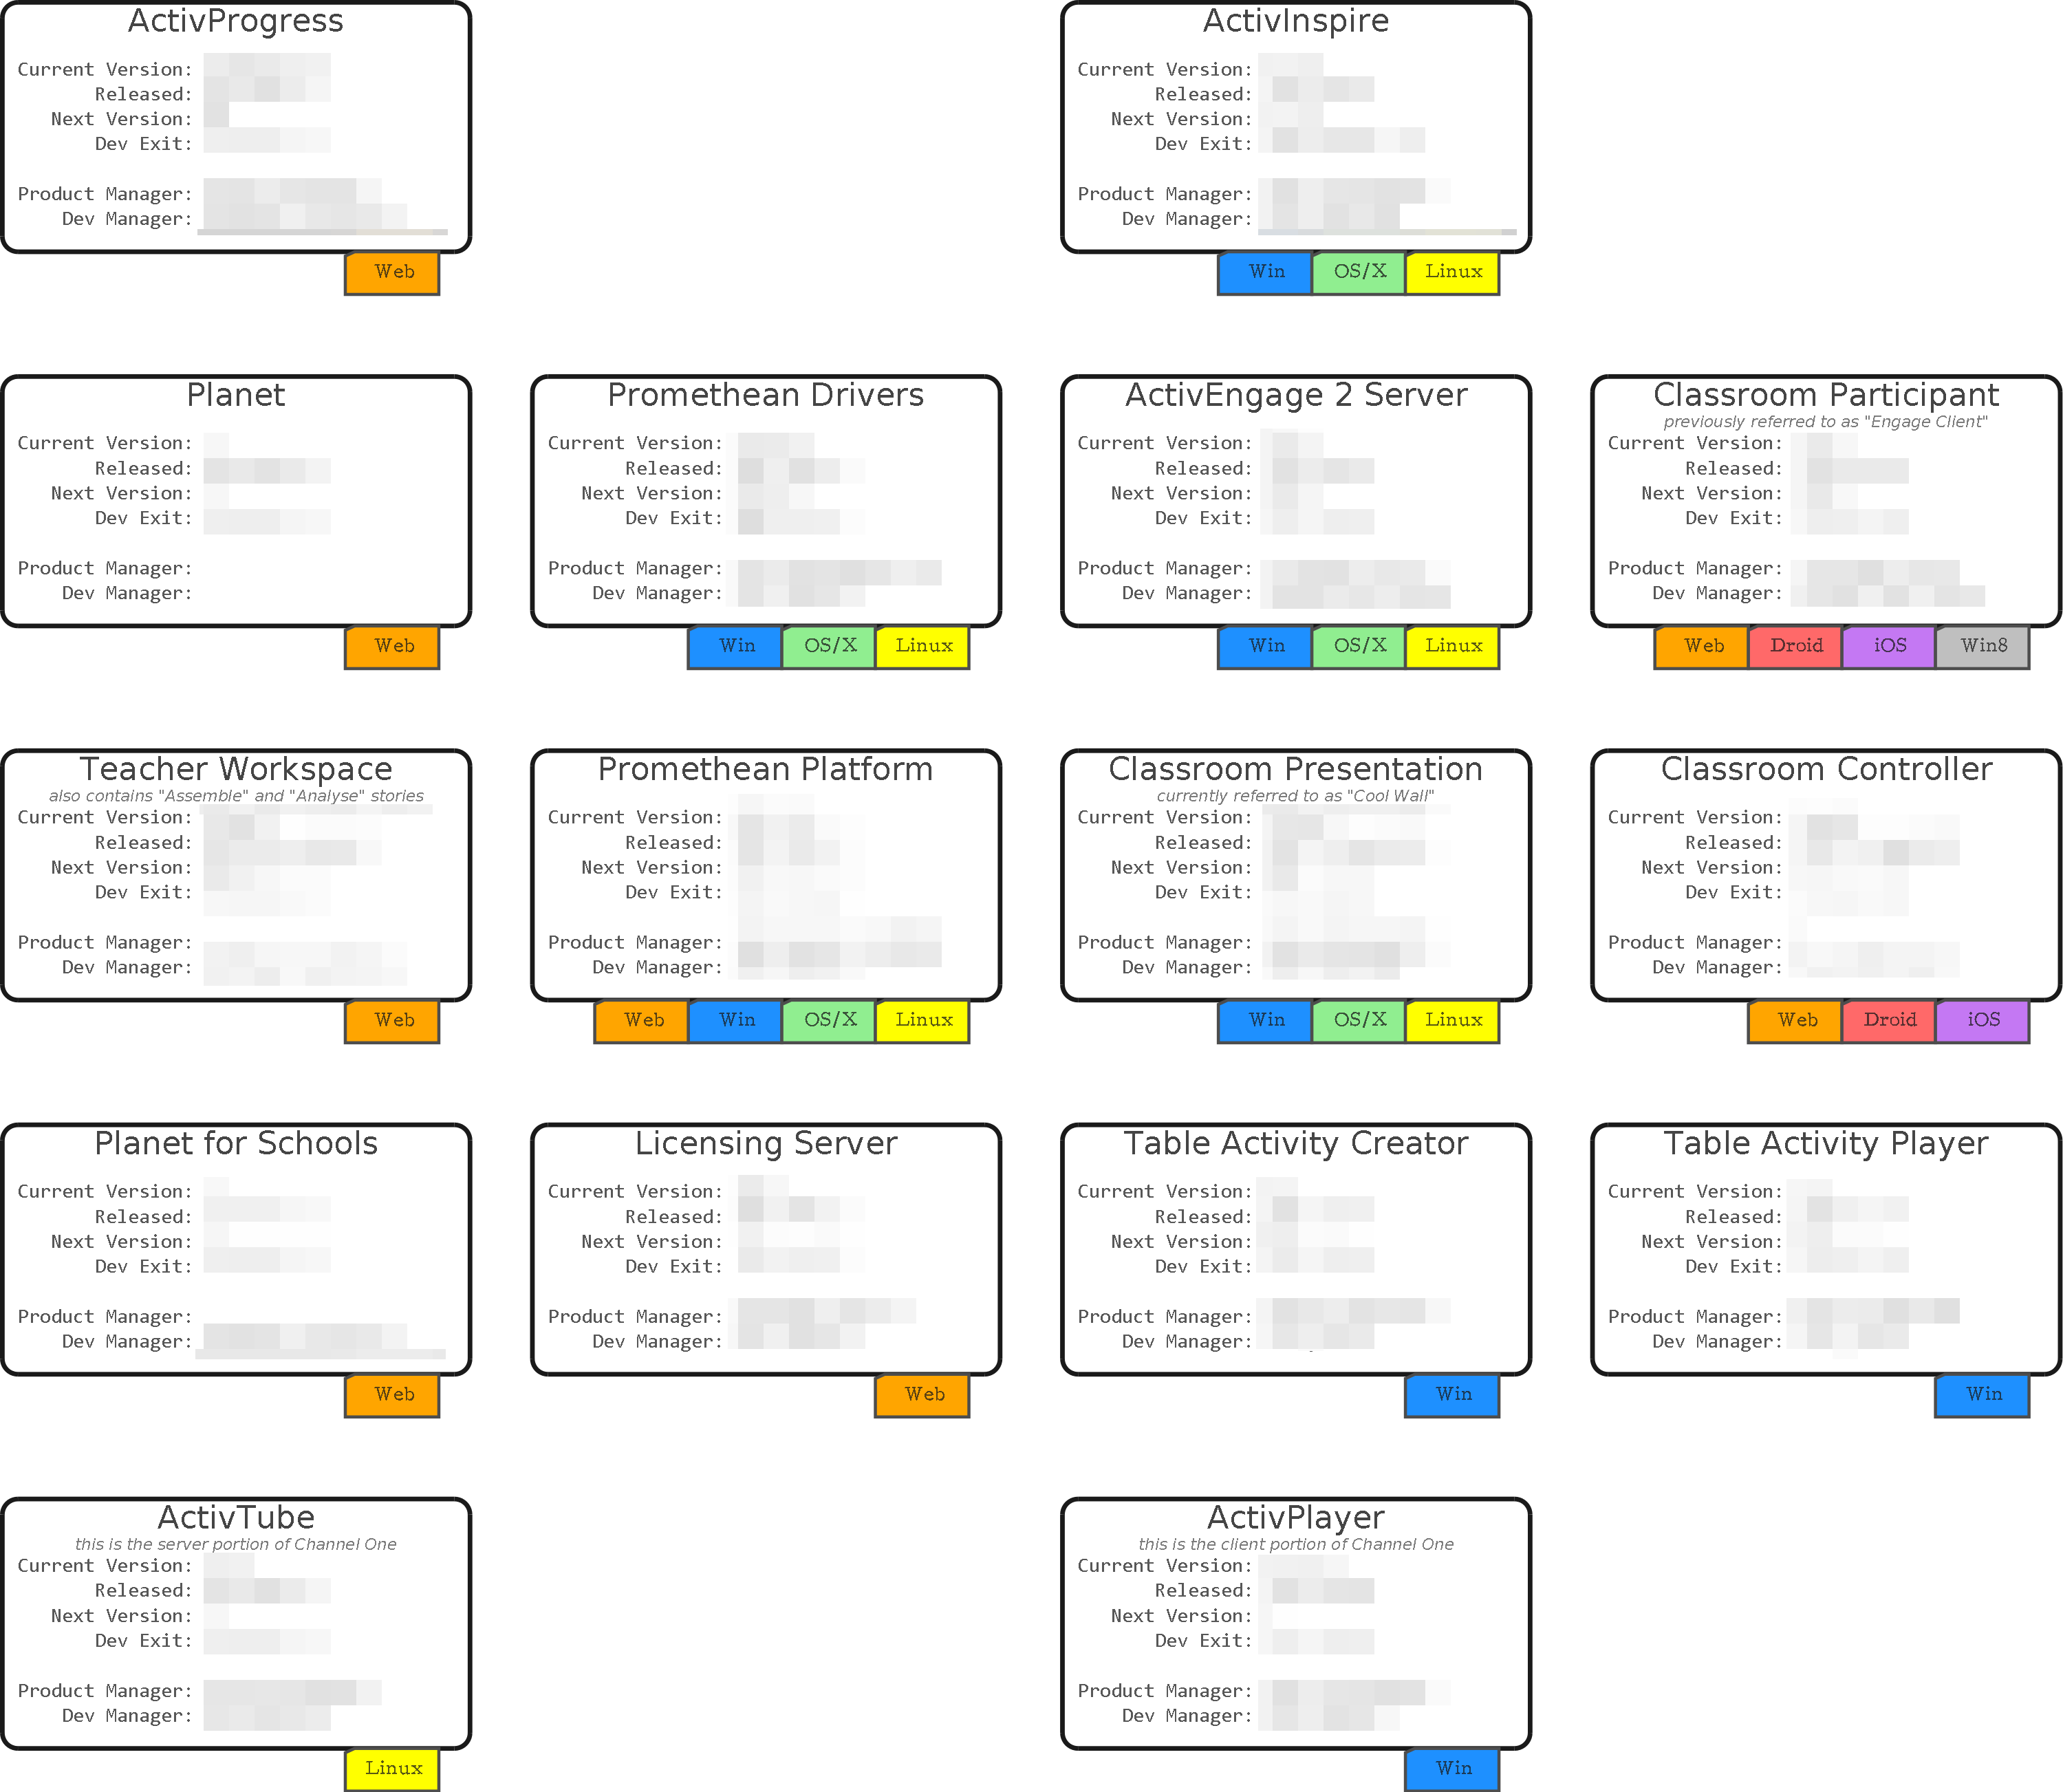
\includegraphics[width=0.8\linewidth]{Prom-ProductMatrix-Clean}
  \caption{The 2013 Product Matrix}
  \label{fig:PromSide}
\end{figure}
\end{centering}

Much of my work at Promethean was entirely strategic\footnote{\href{http://prezi.com/v-jhcxlibwka/?utm_campaign=share&utm_medium=copy&rc=ex0share}{Strategy Council Prezi}\\ http://bit.ly/1bdyeTS}.  I regularly traveled internationally to localize and culturalize our software products.  As well I ushered the global software team through a time of deep organizational change, merging three isolated software divisions as we shifted from one executive regime to another (Promethean had a change of CEO in 2012).  My experience at Promethean, a public global corporation, \pstandout{provided new skills and tools for working in and with large companies}.

\subsection{\textbf{Chief Architect} at \shstandout{SynapticMash LLC} \shyears{[2008-2010]}}
SynapticMash\footnote{\href{http://www.crunchbase.com/company/synapticmash}{SynapticMash on Crunchbase}\\ http://bit.ly/Ls8EVh} was an education software company focused on data analytics, social networking and classroom engagement.  I was hired before investment series A closed.  I designed and built the entire technology organization\footnote{\href{http://synapticmash.com/index.php/about}{The SynapticMash Executive Team}\\ http://bit.ly/1b8NfX3} including software architecture, products and hosting infrastructure.

My responsibilities at SynapticMash included:
\begin{itemize}
\itemsep-0.5em
\item{Hiring the entire software design, development and delivery teams}
\item{Capturing and documenting product specifications}
\item{Defining and documenting software and hosting architecture}
\begin{marginfigure}%
  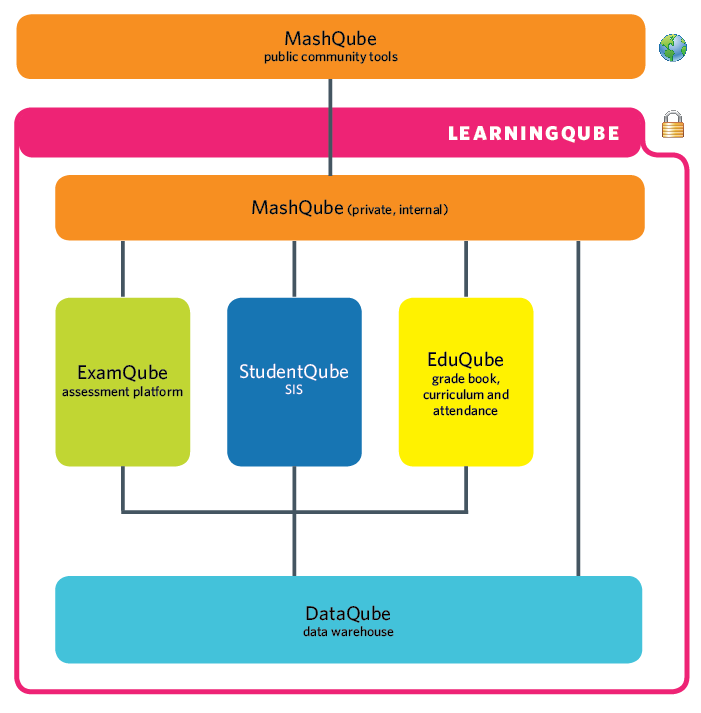
\includegraphics[width=\linewidth]{SM-Product-Architecture}
  \caption{SM Product Architecture}
  \label{fig:SM-Product-Architecture}
\end{marginfigure}
\item{Managing the patent portfolio}
\item{Delivering software products}
\item{Building and maintaining strategic partnerships}
\item{Reporting SDLC progress to investors and the board}
\item{Presenting our technology vision externally at conferences}
\end{itemize}

SynapticMash was my \pstandout{first experience building an organization and delivering products within a venture capital funded company}.  We sold\footnote{\href{http://www.inc.com/news/articles/2010/07/synapticmash-acquired-by-promethean.html}{The SynapticMash Transaction}\\ http://bit.ly/1i7qeeQ} to Promethean, Inc. in 2010 where I continued my executive leadership position.

\subsection{\textbf{CTO \& Cofounder} at \shstandout{Sound Designs LLC} \shyears{[2006-2008]}}
Sound Designs was a New York-based branding, web design, software development and hosting business catering to music companies\footnote{\href{https://web.archive.org/web/20060215201617/http://www.dangelicoguitars.com/guitars.php?}{D'Angelico Guitars Web Site}\\ http://bit.ly/1dwsbwV}, musicians\footnote{\href{https://web.archive.org/web/20070616015006/http://undeadpunk.com/}{The Undead Web Site}\\ http://bit.ly/1adVhDm}, supermodels and visual artists.  We developed an in-house content management and calendaring system tied to a skinnable actionscript streaming audio player to create online presence for bands.  This was my \pstandout{first time dealing with highly internationalized products}-- some\marginnote{With customers such as D'Angelico Guitars, this business was great for growing my guitar collection.} sites had distinct language and culturization requirements when viewed in English, French, Spanish and Arabic.

\subsection{\textbf{CTO \& Founder} at \shstandout{Opus Designs LLC} \shyears{[1997-2008]}}
Opus Designs started as a vehicle for packaging and reselling software and tools I built during my experiences running Office Centers.  Eventually it evolved into a bespoke software company, primarily bringing in revenue via licensable software technologies.  These libraries, products and services most often dealt with large-scale data analytics and scalability.  We used a wide variety of technologies to build bespoke software and specialized systems across many platforms.

\begin{marginfigure}%
  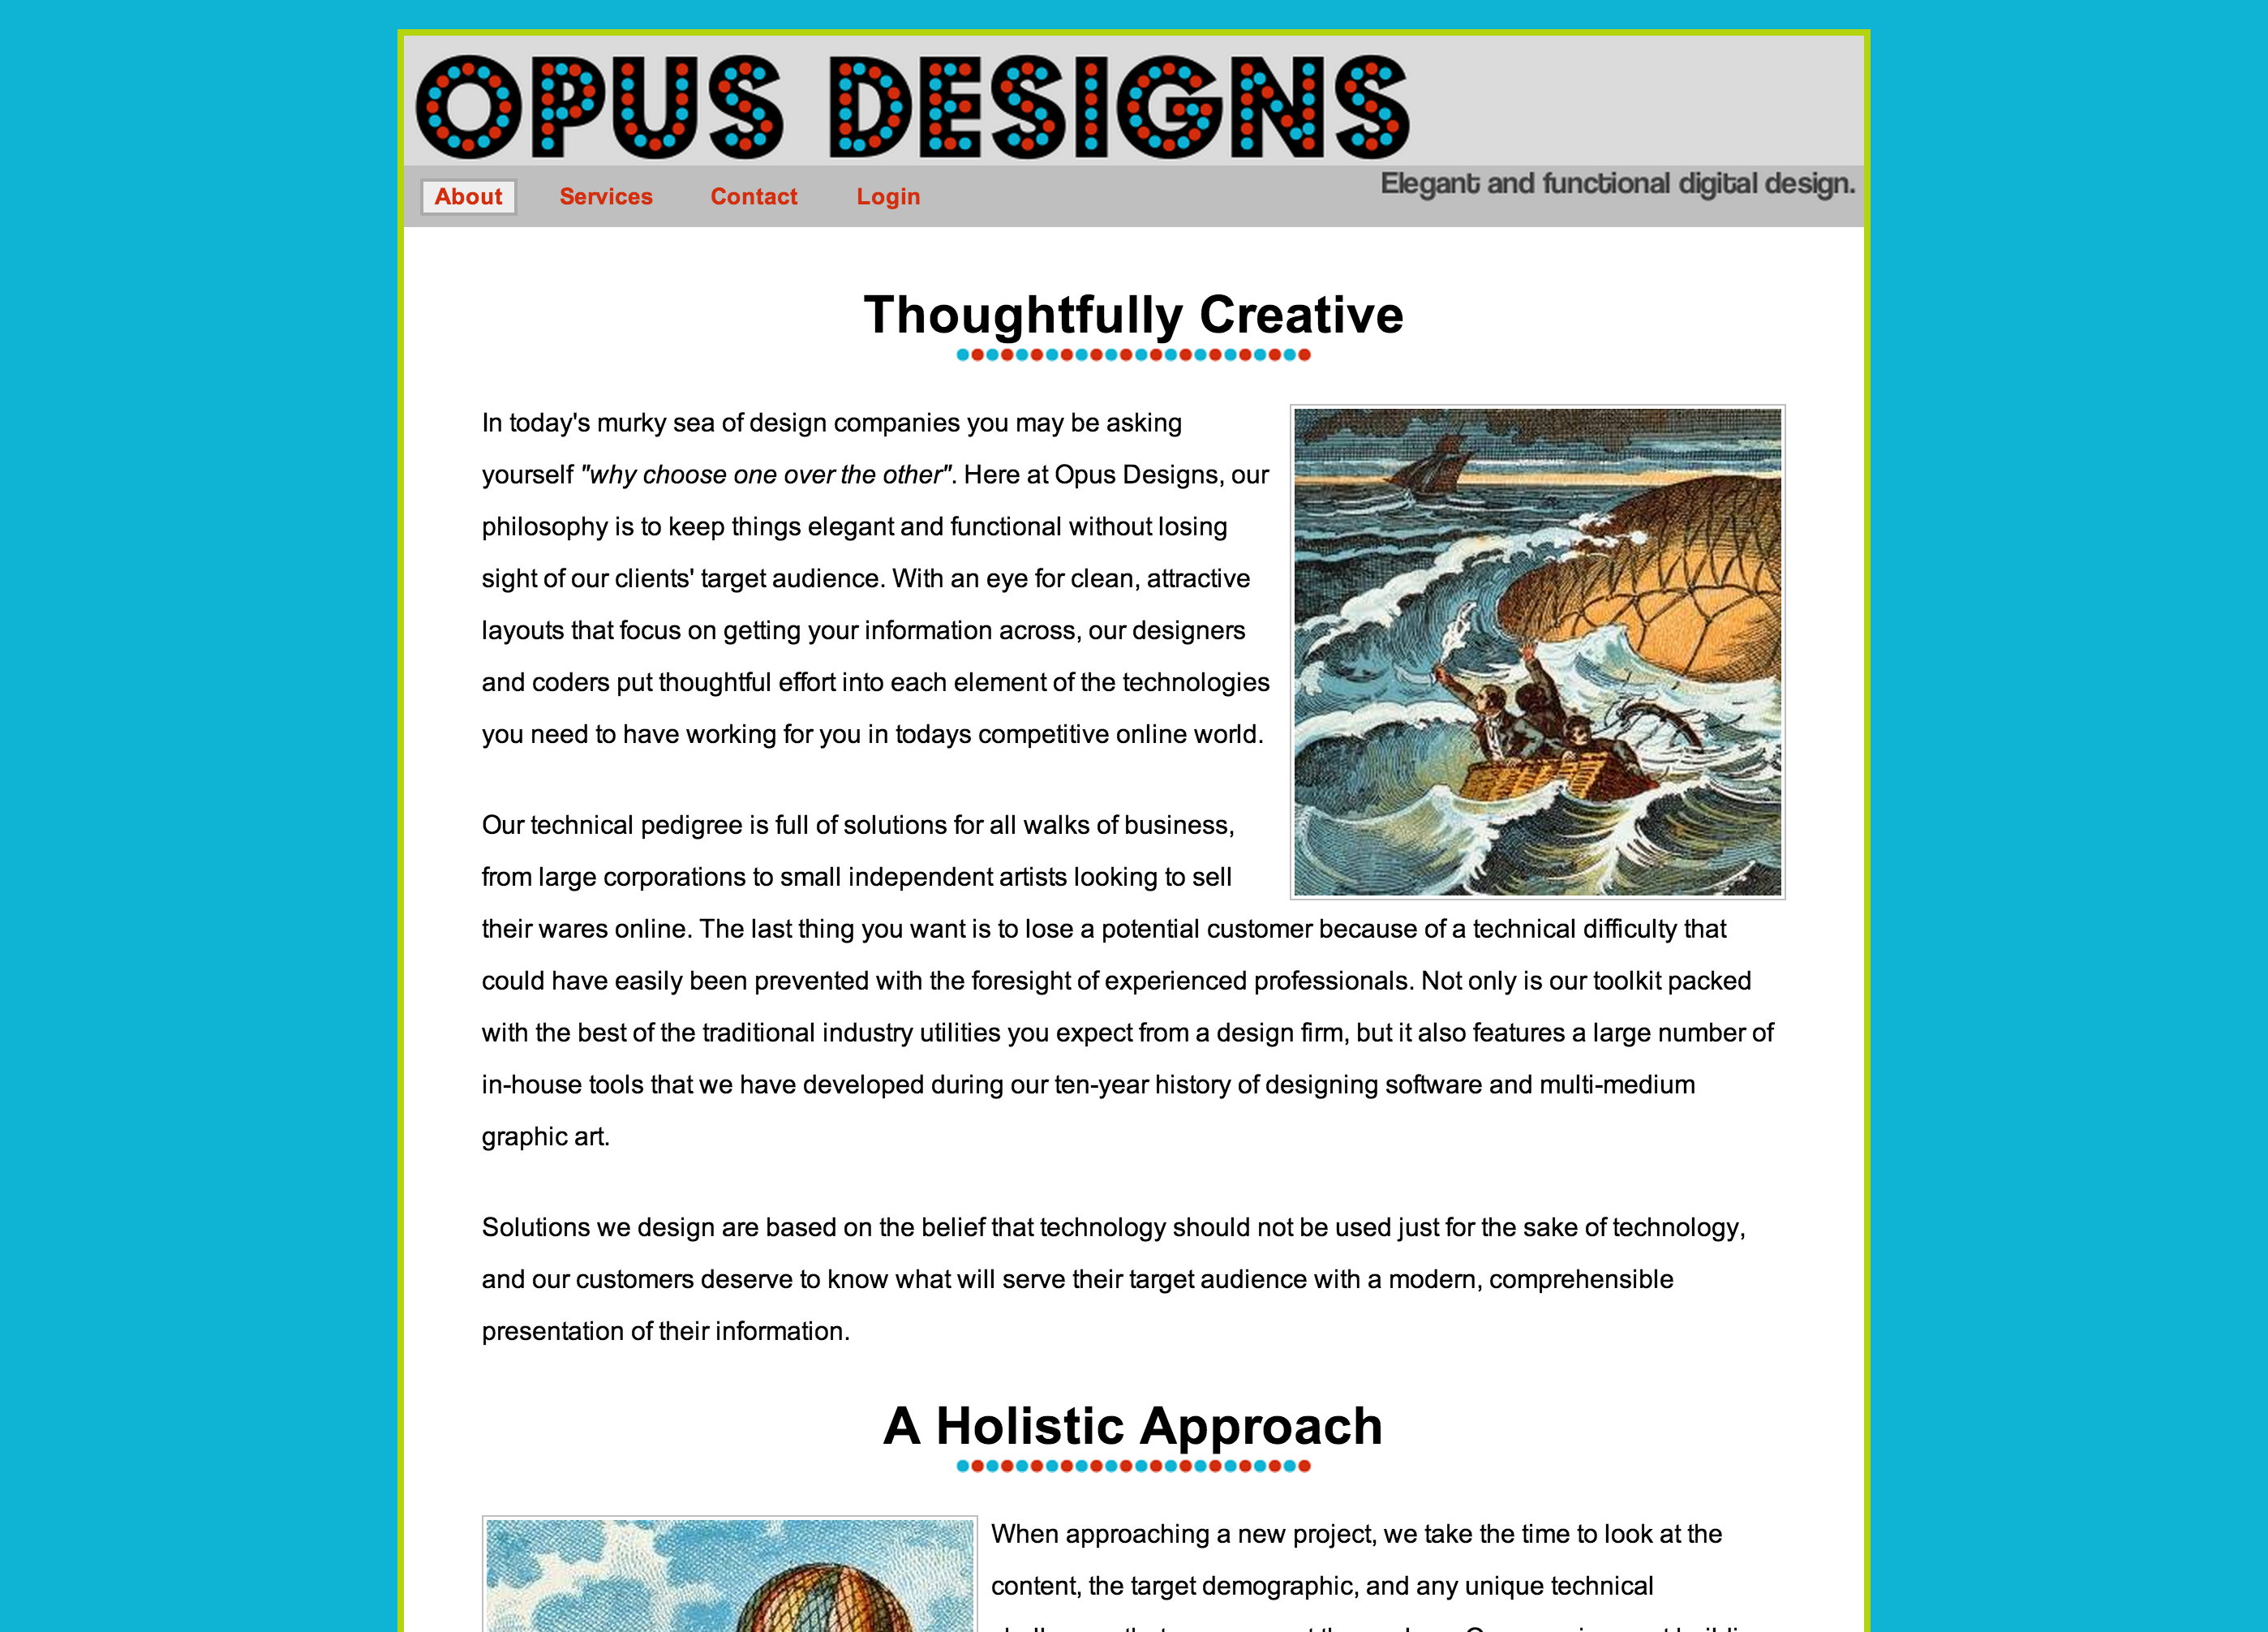
\includegraphics[width=\linewidth]{OpusSite}
  \caption{Opus Designs site 2007}
  \label{fig:OpusSite}
\end{marginfigure}
We billed ourselves as an artisan shop for solving complex problems with technology.  The resulting vertical market software solutions were delivered around recurring revenue licensing models, some as stand-alone applications and others providing SDKs for customers to build upon.  A few of the more interesting problems we solved included:
\begin{itemize}
\itemsep-0.5em
\item{Applying grid solvers to massive databases to compute optimized sales playbooks for broadcast advertising.}
\item{Using GPS\marginnote{Many of these advanced algorithm-based projects were first written in C++, then rewritten in Haskell or Lisp.} and time-of-day drive time statistics to optimize mix levels and agitation speed for material delivery (e.g. cement).}
\item{Delivering emails from queued flat files, allowing legacy software to emit messages to the internet without rewrite.}
\item{Working with internet software companies having trouble scaling their technology and teams.}
\item{Writing custom drivers and interfaces for Linux embedded devices.}
\end{itemize}

The work at Opus Designs allowed me to \pstandout{further understand and hone my ability to intentionally drive a strategic balance between technology management, people management and business model}.

\subsection{\textbf{Vice President \& Cofounder} at \shstandout{Office Centers Inc.} \shyears{[1995-1999]}}
Office Centers was a fully staffed professional services executive suite with offices in Lynnwood, Seattle and Everett.  As the Vice President and Cofounder my time was spent \marginnote{It became evident at this organization that I did not enjoy managing low wage/high turnover staff.  This was the primary reason I moved on.}managing contracts, hiring employees and building technology to keep us ahead of the market.  This was the \pstandout{first organization where my responsibilities included building a team and organizational culture}.

\subsection{\textbf{Graphic Designer} at  \shstandout{MBA Press} \shyears{[1993-1995]}}
MBA Press was a tiny independent printing press near Santa Cruz, California.  My tasks there involved designing print materials, processing imagery in a professional press darkroom and running machinery such as printing presses.  Working in a structured environment like a press with dedicated phases of product \pstandout{gave me a good sense for project and organizational abstraction}.

\subsection{\textbf{Intern, Consultant} at \shstandout{BDI Distributing Inc.} \shyears{[1990-1993]}}
BDI was a small service-oriented computer consultancy\marginnote{Between 1990 and 1993 I had the opportunity to visit and explore Comdex Las Vegas, which in those days was the trade show to be at for learning the technology craft.} with customers all across the Pacific Northwest.  As a networking consultant at BDI Distributing I was tasked with building and configuring IBM PC clones, building and managing LANs and developing custom software.  Of note I \pstandout{designed, developed and shipped my first networked database software in 1992} from BDI: a turn-key replacement for time cards using monochrome touch-screen displays and the Btrieve/Novell database engine.
